\documentclass{article}
\usepackage[utf8]{inputenc}
\usepackage{graphicx}

\title{gEDA and LaTeX}
\author{Shelcia Carolyn Samuvel }
\date{24 April 2020}

\begin{document}

\maketitle

\section{Introduction}
In this document we understand how to create circuits using gschem and stimulate it using ngspice. The main source of work in done using Linux.

\section{Procedure}
1. \textbf{Schematic}: gschem is one of the project of gEDA. The gEDA project has produced and continues working on a full GPL'd suite and toolkit of Electronic Design Automation tools. These tools are used for electrical circuit design, schematic capture, simulation, prototyping, and production. \\
2. \textbf{Circuit description}: gnetlist is the netlist extraction/generation program which is part gEDA (GPL Electronic Design Automation) toolset. This program takes a schematic for its input and outputs a netlist. \\
3. \textbf{Stimulation and Plotting}: Ngspice is a mixed-level/mixed-signal circuit simulator. Its code is based on three open source software packages: Spice3f5, Cider1b1 and Xspice. It is the open source successor of these venerable packages. Many, many modifications, bug fixes and improvements have been added to the code, yielding a stable and reliable simulator. Therefore, besides being used as a standalone simulator, Ngspice has been incorporated into many projects. \\
4. \textbf{Documentation}: Finally, the work is made into a document form(pdf), using latex. LaTeX is a document preparation system for high-quality typesetting. It is most often used for medium-to-large technical or scientific documents but it can be used for almost any form of publishing. Thus, I have prepared this document using Overleaf - Online Latex editor.

\newpage

\section{Schematic}
The circuit is created using gEDA- gschem. The circuit is a voltage divider circuit, consists of 2 resistor in series with a voltage source. \\
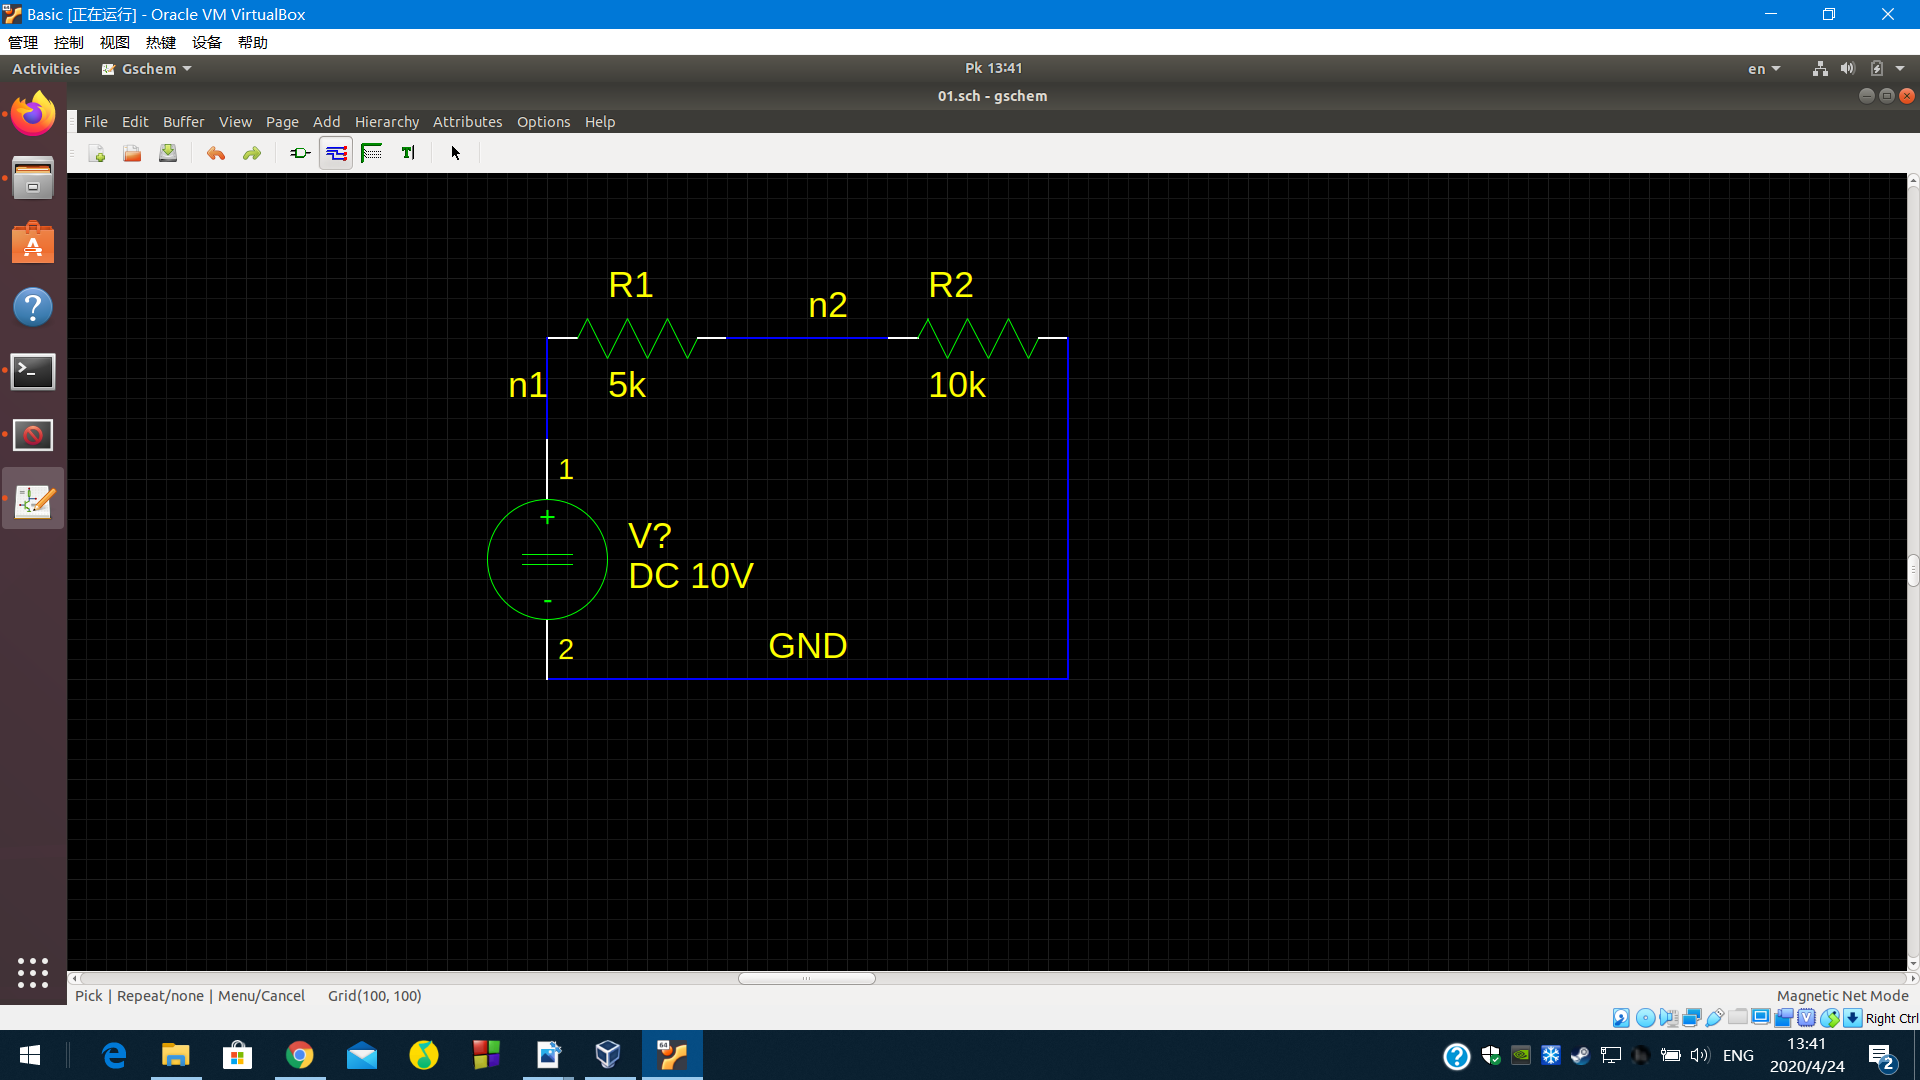
\includegraphics[width=1\textwidth]{sch.png}

\section{Circuit Description and Stimulation}
The description and stimulation is done using Linux terminal. The commands in the terminal are used to describe the circuit, stimulate and plot. The commands in the terminal are shown in the below figure. \\ 
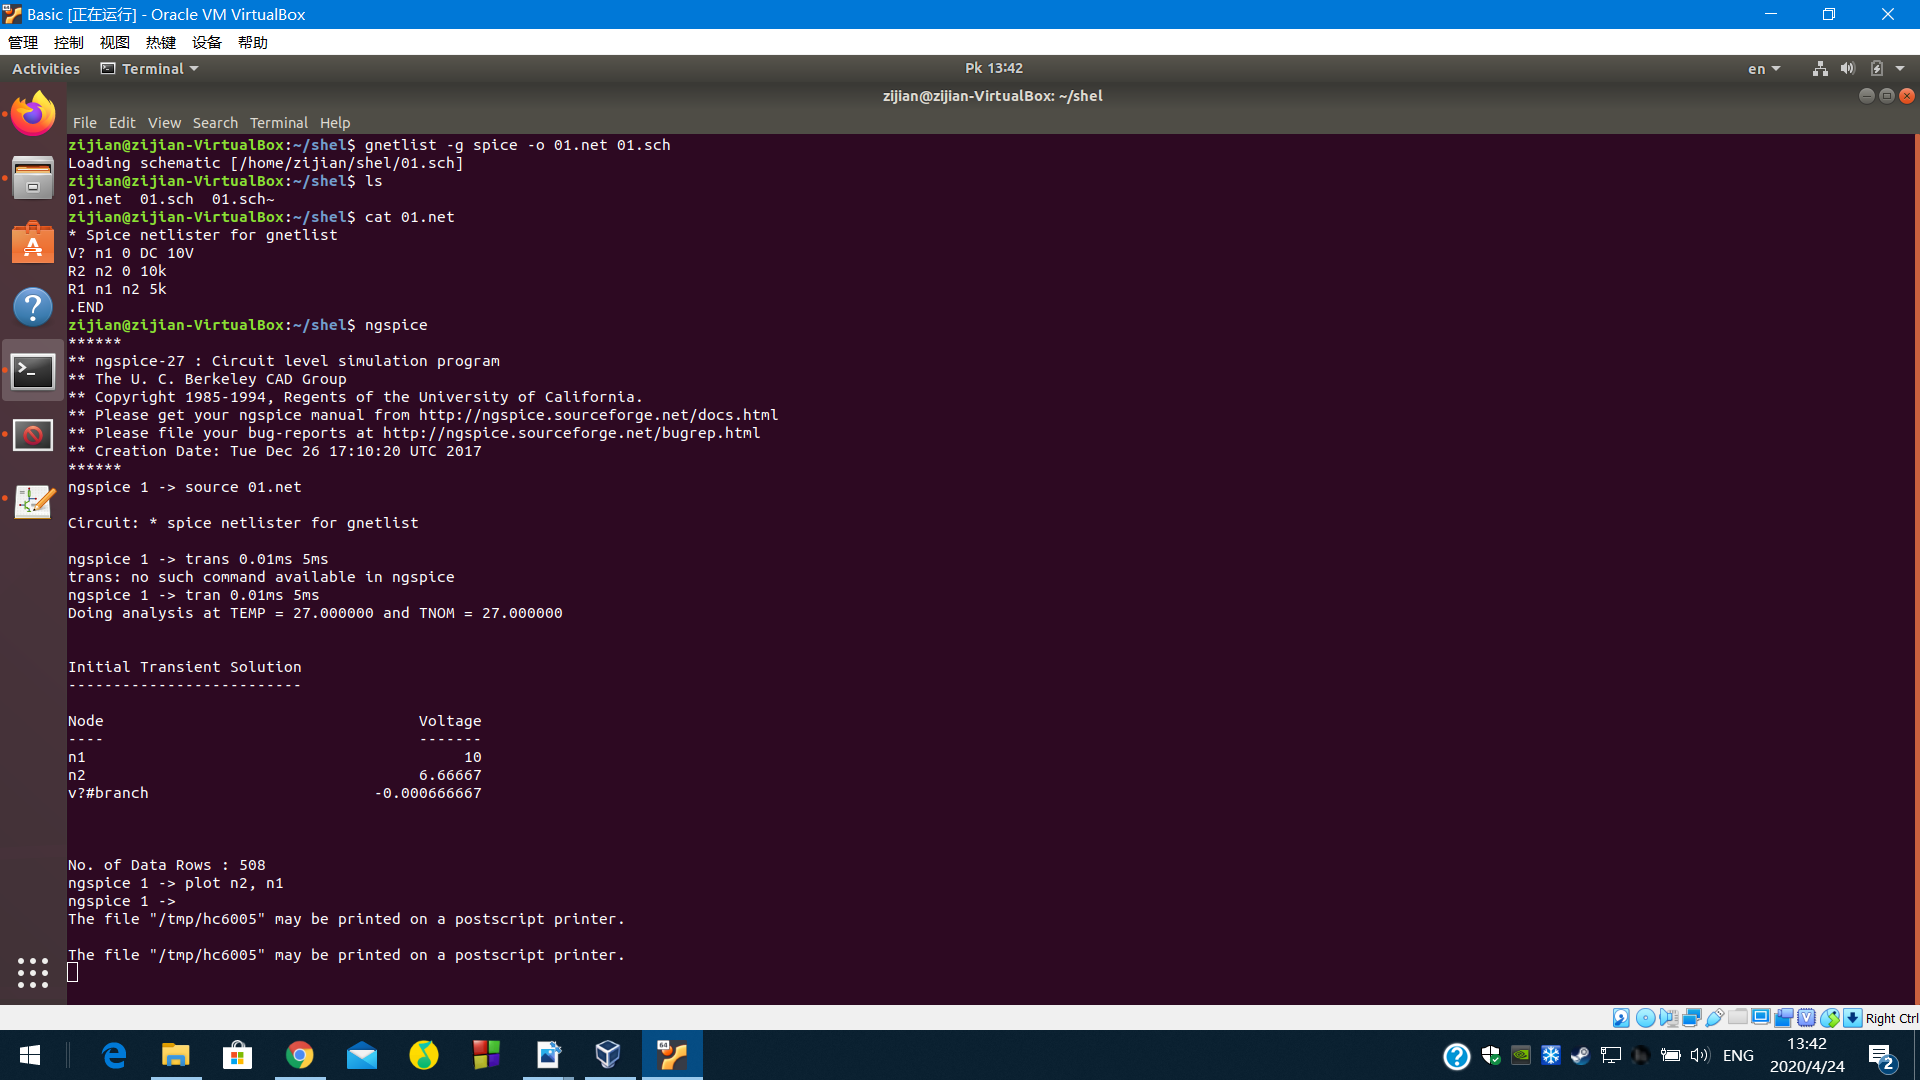
\includegraphics[width=1\textwidth]{terminal.png}

\newpage

\section{Plot}
From the results we can clearly see that the circuit acts as voltage divider. As of we understand from the mathematical calculation the voltage in n1 is 10V because there is no voltage drop; whereas the voltage in n2 is \\ =(DC*R2)/(R1+R2) \\ =(10*10k)/(5k+10k) \\ = 6.66666V \\ because there is a voltage drop in the R1.\\ So, the mathematical calculations and the results obtained using ngspice are the same. The results are plotted and shown in the below figure.\\
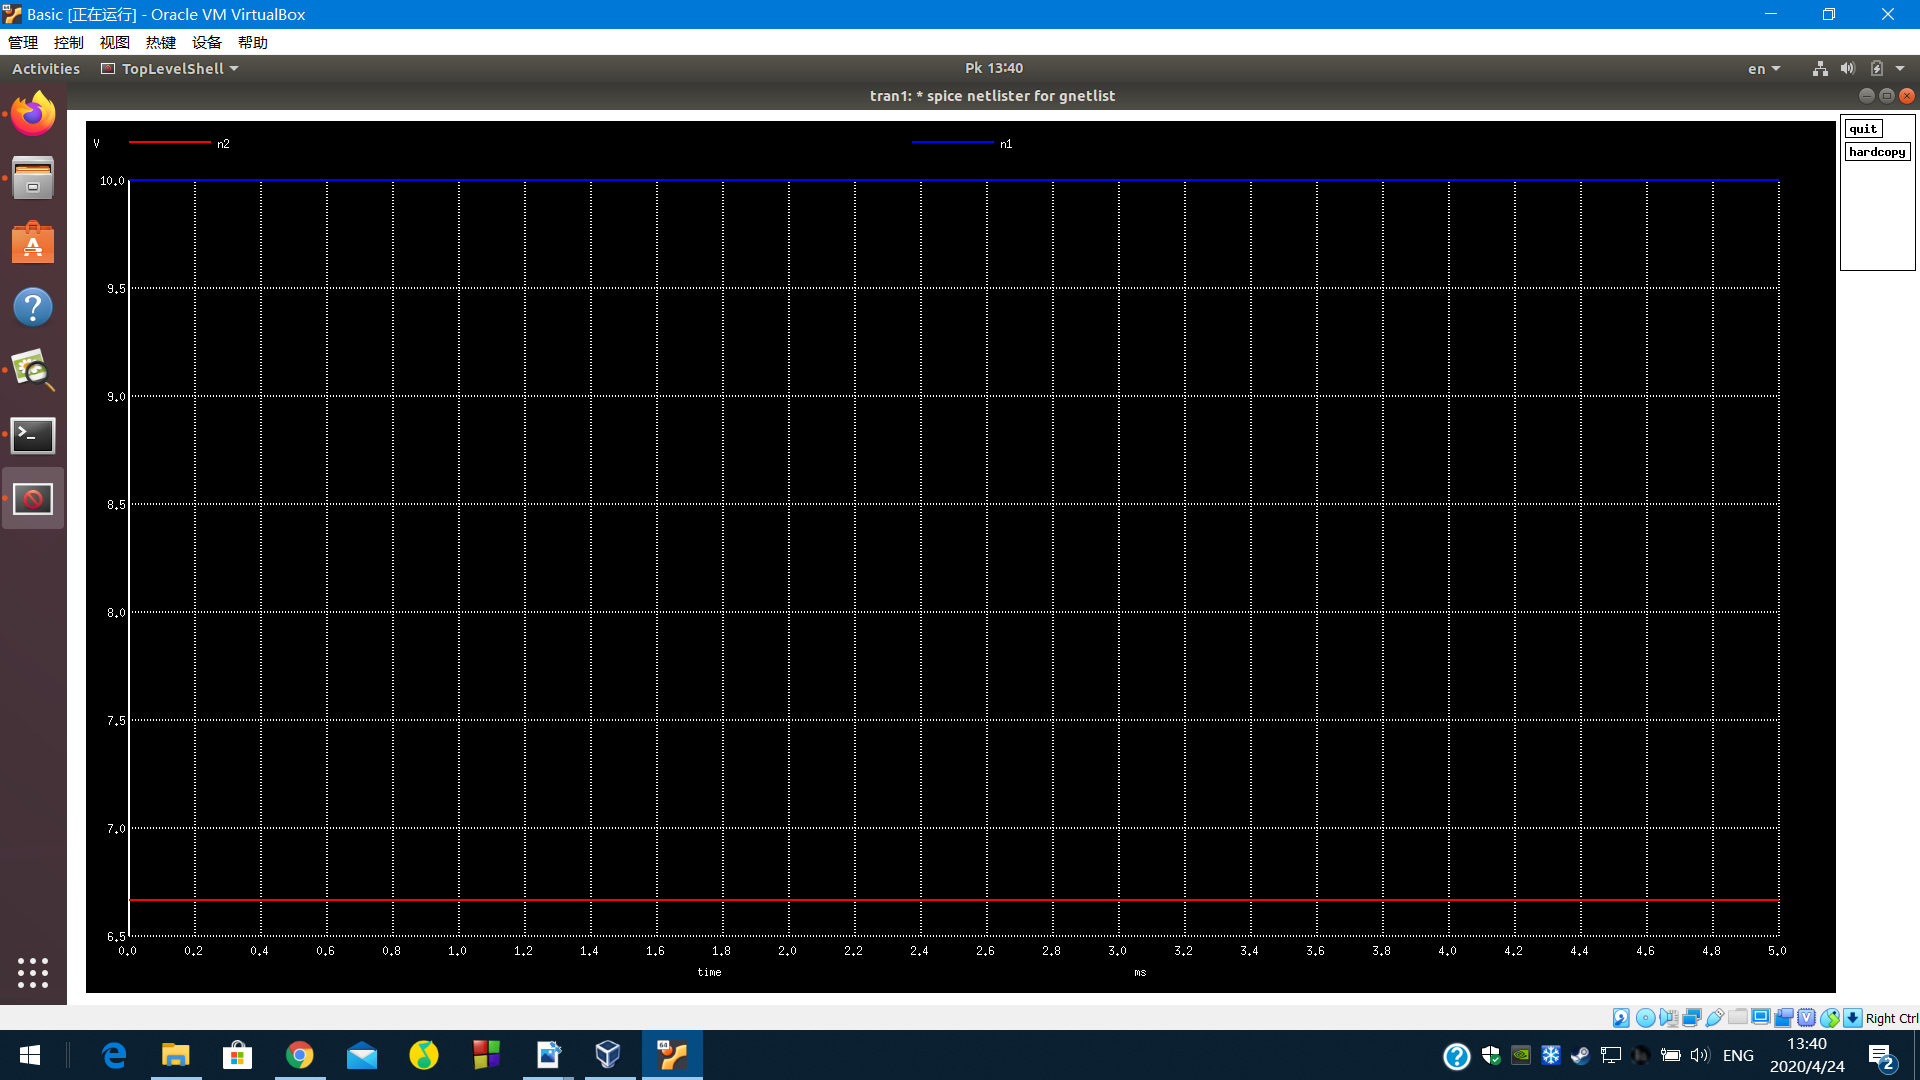
\includegraphics[width=1\textwidth]{plot.png}\\\\\\\\

\centering
\textbf{Thank you!}

\end{document}